% https://github.com/James-Yu/LaTeX-Workshop/wiki/Compile#magic-comments
% !TEX program = xelatex

\documentclass{article}
\usepackage[english,russian]{babel}

% Packages
\usepackage{tabularx}
\usepackage{spverbatim}
\usepackage[hidelinks]{hyperref}

\usepackage{fontspec}
\setmainfont{Go}
\setmonofont{GoMono}

\usepackage{graphicx}
\graphicspath{ {./data/} }

\usepackage{geometry}
\geometry{
 a4paper,
 total={170mm,257mm},
 left=20mm,
 top=20mm,
 }

% Description
\author{Виталий Зарубин}
\title{Пример \LaTeX{}}
\date{\today}

\begin{document}

    % Select language
    \selectlanguage{russian}

    % Title page
    \maketitle

    % New pages
    \newpage
    % Chapter without number
    \section*{О шаблоне}

    Это шаблон \LaTeX{} на русском языке.
    Вы не найдете в шаблоне полной информации по \LaTeX{}, для этого есть специализированные книги.
    Здесь просто набор основных, по моему мнению, конструкций - вся суть в коде.

    % New pages
    \newpage
    % Chapter with number
    \section{Компоненты}

    Многие свалили на WYSIWYG, но по мне это не очень удобная штуковина: зачем надеяться на сторонние приложения, когда можно написать код.
    Причем каждая программа WYSIWYG будет отличаться друг от друга.
    Microsoft Office, например, закрытая и платная.
    Она плотно сидит в умах наших людей, шутка ли - меня заставляли учить её еще в школе (это было давно).
    Хорошо, что я уже тогда знал что есть LibreOffice и смело получил 2-ку по Microsoft Office, оставшись приверженцем Open-Source.

    % Subtitle without number
    \subsection*{Начнем.}

    Если вы оставите пробел между строками, \LaTeX{} сделает новый абзац.
    Прикольная штука \LaTeX{}, совсем как в HTML/CSS.
    Верстаешь свою статью, книгу, презентацию, но вместо сайта на выходе PDF файл.
    Программисту такой подход близок, работаешь в привычной среде.

    % Save format text
    \begin{verbatim}
    Текст, заключенный между
    begin{verbatim} и end{verbatim}
    будет напечатан
    без обработки \LaTeX{}
    \end{verbatim}

    % Save format text with new lines
    \begin{spverbatim}
    // C использованием пакета spverbatim
    // можно смело писать вставки кода.
    void main() {
        print("Hello, World!");
    }
    \end{spverbatim}

    В примере присутствует \texttt{texttt}, который может выделить ключевые слова.
    Еще, как вариант, выделить слово - просто \underline{подчеркнуть} его.
    Окружение \texttt{tabular} позволяет создавать таблицы с автоматическим определением ширины:

    % Center table
    \begin{center}
        \begin{tabular}{c r @{.} l}
            Выражение с $\pi$ &
            \multicolumn{2}{c}{Значение} \\
            \hline
            $\pi$ & 3&1416 \\
            $\pi^{\pi}$ & 36&46 \\
        \end{tabular}
    \end{center}

    Для более прокаченных таблиц можно использовать пакет \texttt{tabularx}.
    На какой-то элемент документа можно добавить ссылку.
    Пробуем добавить ссылку на таблицу \hyperref[tab:just-1]{"Моя таблица"}.

    % Float table with ref
    \begin{table}[!ht]
        \begin{tabularx}{\textwidth}{|X|X|X|}
            \hline
            \multicolumn{3}{|c|}{Моя таблица}   \\ \hline
            column1    & column2    & column3    \\ \hline
        \end{tabularx}
        \caption{Моя таблица}\label{tab:just-1}
    \end{table}

    %% Sub-chapter with number
    \subsection{Подраздел}

    Если \texttt{section} - это глава, то \texttt{subsection} - это подраздел главы.
    Есть еще \texttt{subsubsection}, наверное, это подраздел подраздела.
    В этом подразделе мы добавим цитату, сноску, список, нужные вещи, которые делаются очень просто в \LaTeX{}.

    % Quote with name author
    \begin{quote}
        Интеллект — это способность избегать выполнения работы, но так, чтобы она при этом была сделана.
        \begin{flushright}
            - Линус Торвальдс
        \end{flushright}
    \end{quote}

    Теперь мы сделаем сноску. Для этого мы можем использовать \texttt{footnote}.
    Давайте ее создадим
    % Footnote example
    \footnote{
        И напишем здесь дополнительную информацию о том, как чудесно писать на \LaTeX{} =)
    }

    Добавим небольшое перечисление.
    Обратите внимание, что можно использовать разные символы для перечисления.

    % Lists example
    \begin{enumerate}
        \item Нумерованный список.
        \begin{itemize}
            \item Список в списке.
            \item[-] Список в списке.
            \item[*] Список в списке.
        \end{itemize}
    \end{enumerate}

    % New page
    \newpage
    % Chapter with number
    \section{Установка на Ubuntu 24.04}

    Что нужно сделать для того, чтобы собрать этот шаблон на Ubuntu 24.04 и удобно писать \LaTeX{} код с превью, как мы любим.
    % Footnote example
    \footnote{
        Я расскажу, как это сделал я, на истину в последней инстанции не претендую.
    }

    % Image
    \begin{figure}[h]
        \centering
        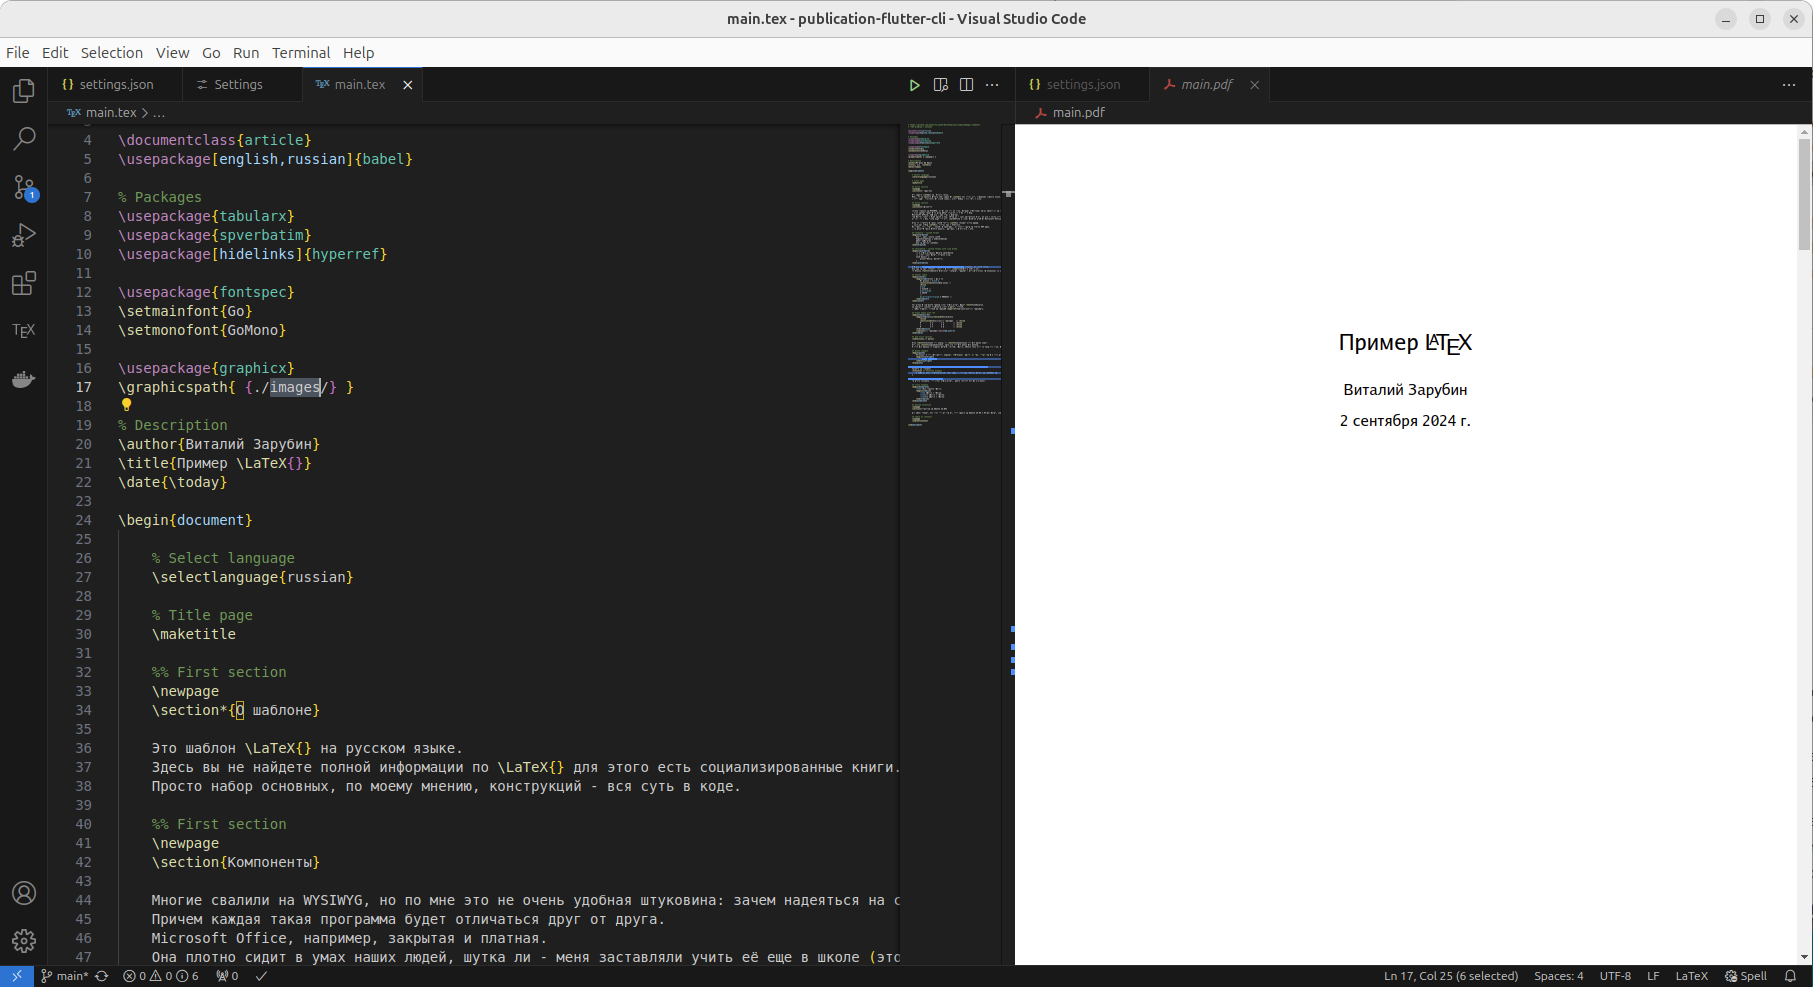
\includegraphics[width=\linewidth]{preview}
        \caption{Превью}
    \end{figure}

    В первую очередь установим Visual Studio Code. Он доступен, бесплатен.
    И у него есть отличное расширение. Переходим на сайт и следуем инструкциям:
    \href{https://code.visualstudio.com}{https://code.visualstudio.com}

    Затем установим расширения vscode:

    % List
    \begin{itemize}
        \item \href{https://marketplace.visualstudio.com/items?itemName=James-Yu.latex-workshop}{LaTeX Workshop}
        \item \href{https://marketplace.visualstudio.com/items?itemName=valentjn.vscode-ltex}{LTeX – LanguageTool grammar/spell checking}
        \item \href{https://marketplace.visualstudio.com/items?itemName=ybaumes.highlight-trailing-white-spaces}{Highlight Trailing White Spaces}
    \end{itemize}

    Подготовим Ubuntu, установив необходимые пакеты одной командой:

    % Save format text with new lines
    \begin{spverbatim}
sudo apt-get install \
    latexmk \
    texlive-xetex \
    texlive-extra-utils \
    texlive-latex-extra \
    texlive-lang-cyrillic \
    texlive-fonts-extra \
    font-manager
    \end{spverbatim}

    Для удобства использования vscode, можно добавить следующие настройки расширения LaTeX Workshop.
    Это включает аннотацию из документа
    % Save format text
    \begin{verbatim}
    % !TEX program = xelatex
    \end{verbatim}
    и настраивает сборку в папку \texttt{build} проекта.

    % Save format text with new lines
    \begin{spverbatim}
    "latex-workshop.latex.build.forceRecipeUsage": false,
    "latex-workshop.latex.outDir": "%DIR%/build",
    "latex-workshop.latex.magic.args": [
        "-synctex=1",
        "-interaction=nonstopmode",
        "-file-line-error",
        "--output-directory=%OUTDIR%",
        "%DOC%"
    ],
    \end{spverbatim}

    Теперь можно писать свою первую статью в \LaTeX{}.
    Это нелегкая прогулка, но освоить базовые вещи не так сложно.
    Если вы разбираетесь в CSS, вы должны примерно представлять с чем будете иметь дело.

    % Top padding
    \vspace{3mm}
    Всем удачи!

    % New page
    \newpage
    % Table of contents
    \tableofcontents

\end{document}
